\subsection{Detection}
\label{sec:eval_req_detection} 

\subsubsection{Configuration}

\begin{figure}[H]
    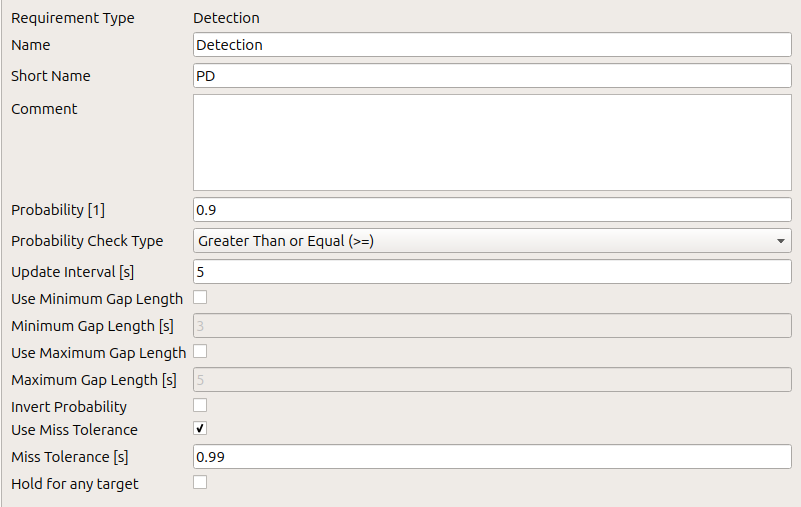
\includegraphics[width=14cm,frame]{figures/eval_req_detection.png}
  \caption{Evaluation Detection requirement}
\end{figure}

The 'Detection' requirement can be used to check whether targets are detected at all. For each target existing in the reference data (within the current sector) a target must be detected within e.g. each test update interval or other given interval. Missed update intervals are either called misses or gaps, which are used to calculate a probability of detection, which has to fulfill a given threshold. \\

\begin{itemize}  
\item Probability [1]: Probability of detection
\item Probability Check Type: $\geq$
\item Update Interval [s]: Update interval of the test data
\item Use Minimum Gap Length: Checkbox if minimum gap length should be used
\item Minimum Gap Length [s]: Minimum gap length to be considered
\item Use Maximum Gap Length: Checkbox if maximum gap length should be used
\item Maximum Gap Length [s]: Maximum gap length to be considered
\item Use Miss Tolerance: Checkbox if miss tolerance should be used
\item Miss Tolerance [s]: Acceptable time delta for miss detection
\item Hold for any Target: Whether the required threshold must hold for any single target (as opposed to the common sector aggregate)
\end{itemize}
\ \\

\subsubsection{Calculation}

As a summary, the reference is used to calculate the number of expected update intervals inside the sector layer (\#EUI). Then, for the test data, if the reference exists at the time, time differences between target reports are checked and the number of misses/gaps are calculated as number of missed update intervals (\#MUI). \\

Gaps are, if a minimum or maximum gap length is used, only counted if the detected gap fulfills the thresholds. \\

The ratio of \#MUI and \#EUI gives the probability of missed update intervals, the counter-probability gives the Probability of Detection (PD). The PD must be greater or equal to the defined 'Probability' for the requirement to pass.

\subsubsection{Result Values}

\paragraph{Sector}

\begin{center}
 \begin{table}[H]
  \begin{tabularx}{\textwidth}{ | l | X |  l | }
    \hline
    \textbf{Name} & \textbf{Description} & \textbf{Example} \\ \hline
    Sector Layer & Name of the sector layer & fir\_cut\_sim \\ \hline
    Requirement Group & Name of the requirement group & Mandatory  \\ \hline
    Requirement & Name of the requirement & Detection  \\ \hline
    Num Results & Total number of results & 728  \\ \hline
    Num Usable Results & Number of usable results & 417  \\ \hline
    Num Unusable Results & Number of unusable results & 311  \\ \hline
    \#Updates/\#EUIs [1] & Total number of update intervals & 7960  \\ \hline
    \#MUIs [1] & Number of missed update intervals & 2221  \\ \hline
    PD [\%] & Probability of Detection & 72.10  \\ \hline
    Condition &  & >= 90.00  \\ \hline
    Condition Fulfilled &  & Failed  \\ \hline
\end{tabularx}
\end{table}
\end{center}

Also, a table is given for all single targets, sorted by PD.

\paragraph{Single Target}

\begin{center}
 \begin{table}[H]
  \begin{tabularx}{\textwidth}{ | l | X |  l | }
    \hline
    \textbf{Name} & \textbf{Description} & \textbf{Example} \\ \hline
    Use & To be used in results & true \\ \hline
    \#EUIs [1] & Expected Update Intervals & 6 \\ \hline
    \#MUIs [1] & Missed Update Intervals & 5 \\ \hline
    PD [\%] & Probability of Detection & 16.67 \\ \hline
    Reference Period 0 & Time inside sector & [15:47:22.680,15:47:45.828] \\ \hline
    Reference Period 1 & Time inside sector & [15:47:53.844,15:47:57.844] \\ \hline
    Condition &  & >= 90.00 \\ \hline
    Condition Fulfilled &  & Failed \\ \hline
\end{tabularx}
\end{table}
\end{center}
